\documentclass[12pt,a4paper, france]{article}

\newcommand{\workingDate}{\textsc{\selectlanguage{francais}\today}}
\newcommand{\userName}{DM 1}
\newcommand{\institution}{M2 AMI2B}
\newcommand\tab[1][1cm]{\hspace*{#1}}
\usepackage{researchdiary_png}


\begin{document}

\begin{center}
{\textbf {\huge Informatique Théorique}}\\[5mm]
{\large Auguste Gardette} \\[5mm]
{\text{ 14 Octobre 2022}} \\ [5mm]
\end{center}


\section{Exercice 1.}

Soit L le langage des mots sur l’alphabet {a, c, g, t} qui commencent par atg
et finissent par taa. \\

\textbf{1.} Donnez une expression rationnelle de L. \\

\tab atg (a | c | g | t)* taa \\

\textbf{2.} On dit qu\textquoteright un automate A =$<$ A, Q, q${_0}$, F, ${\delta}$ $>$ est d\'eterministe s\textquoteright il satisfait les deux conditions suivantes : \\
\tab — Il ne contient pas d\textquoteright ${\epsilon}$-transition. \\
\tab — Pour tout  \'etat q ${\in}$ Q et toute lettre a ${\in}$ A, il existe au maximum une transition\\

(a) Construisez un automate fini non d\'eterministe \`a sept  \'etats pour L.\\

\begin{tikzpicture}[auto, node distance=1.5cm,semithick, main/.style = {draw, circle}]
\tab \node[main] (1) {0}; 
\node[main] (2) [right of=1] {1}; 
\node[main] (3) [right of=2] {2}; 
\node[main] (4) [right of=3] {3}; 
\node[main] (5) [right of=4] {4}; 
\node[main] (6) [right of=5] {5}; 
\node[main] (7) [right of=6] {6};
\node (8) [right of=7] {}; 
\node (9) [left of=1] {}; 
\path [->]  (1) edge node {a} (2)
(2) edge node {t} (3)
(3) edge node {g} (4)
(4) edge [loop above] node {a,c,g,t} (4)
(4) edge node {t} (5)
(5) edge node {a} (6)
(6) edge node {a} (7)
(7) edge node {} (8)
(9) edge node {} (1)
\end{tikzpicture} \\ [5mm]

(b) Construisez un automate fini d\'eterministe \`a sept  \'etats pour L\\

\begin{tikzpicture}[auto, node distance=1.5cm,semithick, main/.style = {draw, circle}]
\tab \node[main] (1) {0}; 
\node[main] (2) [right of=1] {1}; 
\node[main] (3) [right of=2] {2}; 
\node[main] (4) [right of=3] {3}; 
\node[main] (5) [right of=4] {4}; 
\node[main] (6) [right of=5] {5}; 
\node[main] (7) [right of=6] {6};
\node (8) [right of=7] {}; 
\node (9) [left of=1] {}; 
\path [->]  (1) edge node {a} (2)
(2) edge node {t} (3)
(3) edge node {g} (4)
(4) edge [loop above] node {a,c,g} (4)
(4) edge [bend left=10] node {t} (5)
(5) edge [bend left=10] node {a} (6)
(5) edge [bend left=10] node {c,g} (4)
(5) edge [loop above] node {t} (5)
(6) edge [bend left=10] node {t} (5)
(6) edge [bend left=60] node {c,g} (4)
(6) edge node {a} (7)
(7) edge [bend left=80] node {a,c,g} (4)
(7) edge [bend right=60] node {t} (5)
(7) edge node {} (8)
(9) edge node {} (1)
\end{tikzpicture} \\

\section{Exercice 2.}

Soit la grammaire G suivante : \\

\tab \tab \tab \fbox{
\begin{minipage}[c]{6cm}
S ${\rightarrow}$ aSu | uSa | cSg | gSc| SS | T \\
T ${\rightarrow}$ aT | cT | gT | uT | \epsilon ε
\end{minipage}
}\\

\textbf{1.} Montrez que L(G) = \{a, c, g, u\}${^\text{*}}$\\


Simplifions la grammaire G comme suit : \\

\tab \tab \tab \fbox{
\begin{minipage}[c]{4.8cm}
S → SS | T \\
T → aT | cT | gT | uT | ${\epsilon}$
\end{minipage}
}\\

On peut construire un pseudo automate correspondant : \\

\begin{tikzpicture}[auto, node distance=2cm,semithick, main/.style = {draw, circle}]
\tab \tab \tab \tab \node[main] (1) {0}; 
\node[main] (2) [above of=1] {1}; 
\node[main] (3) [right of=1] {2}; 
\node[main] (4) [above of=3] {3}; 
\node[main] (5) [right of=4] {4}; 
\node[main] (6) [below of=3] {5}; 
\node[main] (7) [right of=6] {6};
\node (8) [right of=3] {}; 
\node (9) [left of=1] {}; 
\path [->]  
(1) edge [bend left=10] node {S} (2)
(2) edge [bend left=10] node {S} (1)
(1) edge node {T} (3)
(3) edge [bend left=7] node {a} (4)
(4) edge [bend left=7] node {T} (3)
(3) edge [bend left=-7] node {c} (5)
(5) edge [bend left=20] node {T} (3)
(3) edge [bend left=7] node {g} (6)
(6) edge [bend left=7] node {T} (3)
(3) edge [bend left=20] node {u} (7)
(7) edge [bend left=-7] node {T} (3)
(3) edge node {} (8)
(9) edge node {} (1)
\end{tikzpicture} \\

En simplifiant on obtient: \\

\begin{tikzpicture}[auto, node distance=2cm,semithick, main/.style = {draw, circle}]
\tab \tab \tab \tab \tab \node[main] (1) {0}; 
\node (2) [right of=1] {}; 
\node (3) [left of=1] {}; 
\path [->]  
(1) edge [loop above] node {a,c,g,u} (=1)
(1) edge node {} (2)
(3) edge node {} (1)
\end{tikzpicture} \\

Grossi\`erement on pouurait m${\hat{e}}$me simplifier la grammaire en ne gardant que : \\ 
\tab T ${\rightarrow}$ aT $|$ cT $|$ gT $|$ uT $|$ ${\epsilon}$. Avec cette grammaire on peut commencer avec n\textquoteright importe quelle lettre, lui incr\'ementer n\textquoteright importe quelle lettre et finir par n\textquoteright importe quelle lettre. \\

\textbf{2.} On dit qu\textquoteright une grammaire G est ambig\"ue s\textquoteright il existe un mot \textit{w} ${\in}$ L(G) qui peut ${\hat{e}}$tre g\'en\'er\'e par au moins deux arbres de d\'erivation dont la racine est l\textquoteright axiome. Montrez
que G est ambigu\"e, en consid\'erant les arbres de d\'erivation qui g\'en\`erent le mot \textit{au}. \\

Voici quelques exemples d'arbres pour former le mot \textit{au} : \\

\begin{tikzpicture}[node distance=1.4cm,semithick, main/.style = {draw}]
\node (1) {S}; 
\node (2) [below left of=1] {S}; 
\node (3) [below right of=1] {S}; 
\node (4) [below of=2] {T}; 
\node (5) [below of=3] {T}; 
\node (6) [below of=4] {T};
\node (7) [left of=6] {\textbf{a}}; 
\node (8) [below of=5] {\textbf{u}}; 
\node (9) [right of=8] {T};
\node (10) [below of=6] {${\epsilon}$}; 
\node (11) [below of=9] {${\epsilon}$};
\node (12) [right of=1] {};
\node (13) [right of=12] {};
\node (14) [right of=13] {};
\node (16) [right of=14] {S};
\node (17) [below of=16] {T};
\node (18) [below left of=17] {\textbf{a}};
\node (19) [below right of=17] {T};
\node (20) [below left of=19] {\textbf{u}};
\node (21) [below right of=19] {T};
\node (22) [below of=21] {${\epsilon}$};
\node (23) [right of=16] {};
\node (24) [right of=23] {};
\node (25) [right of=24] {};
\node (a) [right of=25] {S};
\node (b) [below of=a] {S}; 
\node (c) [left of=b] {\textbf{a}}; 
\node (d) [right of=b] {\textbf{u}}; 
\node (e) [below of=b] {T}; 
\node (f) [below of=e] {${\epsilon}$}; 
\path [->]  (1) edge node {} (2)
(1) edge node {} (3)
(2) edge node {} (4)
(3) edge node {} (5)
(4) edge node {} (6)
(4) edge node {} (7)
(5) edge node {} (8)
(5) edge node {} (9)
(6) edge node {} (10)
(9) edge node {} (11)
(16) edge node {} (17)
(17) edge node {} (18)
(17) edge node {} (19)
(19) edge node {} (20)
(19) edge node {} (21)
(21) edge node {} (22)
(a) edge node {} (b)
(a) edge node {} (c)
(a) edge node {} (d)
(b) edge node {} (e)
(e) edge node {} (f)
\end{tikzpicture}\\

En r\'ealit\'e, avec la possibilit\'e de faire S ${\rightarrow}$ SS, on peut g\'en\'erer une infinit\'e d\textquoteright  arbres pour former le mot \textit{au}, voir n\textquoteright importe quel mot du langage L(G) = \{a, c, g, u\}${^\text{*}}$. On peut raisonnablement dire que la grammaire G est ambig\"ue.\\

\textbf{3.} Soit le mot \textit{cccaaaggguuu}. Montrez que, parmi tous les arbres de d\'erivation menant
\`a ce mot depuis l\textquoteright axiome, il y en a exactement deux qui utilisent trois fois une r\`egle
du type \\ S ${\rightarrow}$ xSy et qui utilisent une fois la r\`egle S ${\rightarrow}$ SS. Dessinez ces deux arbres. \\

\textbf{Arbre 1:} \\

\begin{tikzpicture}[node distance=1.2cm,semithick, main/.style = {draw}]
\tab \tab \tab \node (1) {S}; 
\node (21) [below left of=1] {S}; 
\node (22) [below right of=1] {S};
\node (31) [below of=21] {\textbf{g}};
\node (32) [left of=31] {S}; 
\node (33) [left of=32] {\textbf{c}};
\node (41) [below of=32] {S};
\node (42) [left of=41] {\textbf{c}}; 
\node (43) [right of=41] {\textbf{g}}; 
\node (51) [below of=41] {S};
\node (52) [left of=51] {\textbf{c}}; 
\node (53) [right of=51] {\textbf{g}}; 

\node (61) [below of=51] {T};
\node (71) [below left of=61] {\textbf{a}};
\node (72) [below right of=61] {T};
\node (81) [below left of=72] {\textbf{a}};
\node (82) [below right of=72] {T};
\node (91) [below left of=82] {\textbf{a}};
\node (92) [below right of=82] {T};
\node (101) [below of=92] {${\epsilon}$};

\node (34) [below of=22] {T};
\node (44) [below left of=34] {\textbf{u}};
\node (45) [below right of=34] {T}; 
\node (54) [below left of=45] {\textbf{u}};
\node (55) [below right of=45] {T}; 
\node (64) [below left of=55] {\textbf{u}};
\node (65) [below right of=55] {T}; 
\node (74) [below of=65] {${\epsilon}$};
\path [->]  (1) edge node {} (21)
(1) edge node {} (22)
(21) edge node {} (31)
(21) edge node {} (32)
(21) edge node {} (33)
(32) edge node {} (41)
(32) edge node {} (42)
(32) edge node {} (43)
(41) edge node {} (51)
(41) edge node {} (52)
(41) edge node {} (53)
(51) edge node {} (61)
(61) edge node {} (71)
(61) edge node {} (72)
(72) edge node {} (81)
(72) edge node {} (82)
(82) edge node {} (91)
(82) edge node {} (92)
(92) edge node {} (101)
(22) edge node {} (34)
(34) edge node {} (44)
(34) edge node {} (45)
(45) edge node {} (54)
(45) edge node {} (55)
(55) edge node {} (64)
(55) edge node {} (65)
(65) edge node {} (74)
\end{tikzpicture}\\

\textbf{Arbre 2:} \\

\begin{tikzpicture}[node distance=1.2cm,semithick, main/.style = {draw}]
\tab \tab \tab \tab \node (1) {S}; 
\node (21) [below left of=1] {S}; 
\node (22) [below right of=1] {S};
\node (200) [below of=21] {T}; 
\node (31) [below of=200] {T}; 
\node (32) [left of=31] {\textbf{c}};
\node (41) [below of=31] {T}; 
\node (42) [left of=41] {\textbf{c}};
\node (51) [below of=41] {T}; 
\node (52) [left of=51] {\textbf{c}};
\node (61) [below of=51] {${\epsilon}$};
\node (33) [below of=22] {\textbf{a}}; 
\node (34) [right of=33] {S};
\node (35) [right of=34] {\textbf{u}};
\node (43) [below of=34] {S}; 
\node (44) [left of=43] {\textbf{a}};
\node (45) [right of=43] {\textbf{u}}; 
\node (53) [below of=43] {S}; 
\node (54) [left of=53] {\textbf{a}};
\node (55) [right of=53] {\textbf{u}}; 
\node (62) [below of=53] {T};
\node (71) [below left of=62] {\textbf{g}};
\node (72) [below right of=62] {T};
\node (81) [below left of=72] {\textbf{g}};
\node (82) [below right of=72] {T}; 
\node (91) [below left of=82] {\textbf{g}};
\node (92) [below right of=82] {T}; 
\node (101) [below of=92] {${\epsilon}$};
\path [->]  (1) edge node {} (21)
(1) edge node {} (22)
(21) edge node {} (200)
(200) edge node {} (31)
(200) edge node {} (32)
(31) edge node {} (41)
(31) edge node {} (42)
(41) edge node {} (51)
(41) edge node {} (52)
(51) edge node {} (61)

(22) edge node {} (33)
(22) edge node {} (34)
(22) edge node {} (35)
(34) edge node {} (43)
(34) edge node {} (44)
(34) edge node {} (45)
(43) edge node {} (53)
(43) edge node {} (54)
(43) edge node {} (55)

(53) edge node {} (62)
(62) edge node {} (71)
(62) edge node {} (72)
(72) edge node {} (81)
(72) edge node {} (82)
(82) edge node {} (91)
(82) edge node {} (92)
(92) edge node {} (101)

\end{tikzpicture} ${\\}$

Si on veut respecter la r\`egle S ${\rightarrow}$ SS, l\textquoteright uinque solution est de la placer au d\'ebut puisqu\textquoteright aucune r\`egle de S n\textquoteright est de la forme cSu donc rien ne peut substituer SS pour le premier coup. \\

Puis, si l\textquoteright on souhait respecter la r\`egle 'trois fois S ${\rightarrow}$' xSy, nous somme oblig\'e d\textquoteright utiliser les r\`egles cSg (pour le premier S) ou aSu (pour le second S) trois fois d'affil\'es pour r\'eprondre \`a cette contrainte. Il n\textquoteright y a donc bien que 2 solutions d\textquoteright arbre possible. \\

\textbf{4.} Chacun de ces arbres de d\'erivation correspond \`a une structure secondaire qui peut
${\hat{e}}$tre adopt\'ee par la s\'eequence d’ARN\textit{cccaaaggguuu}. Dessinez les deux structures
secondaires correspondant respectivement \`a chacun des deux arbres. \\

\textbf{Arbre 1 - } Structure secondaire: \tab \textbf{Arbre 2 - } Structure secondaire: \\\

\begin{tikzpicture}[node distance=0.6cm,semithick, main/.style = {draw}]
\tab \tab \tab \node (1) {u}; 
\node (2) [below of=1] {u}; 
\node (3) [below of=2] {u}; 
\node (4) [below of=3] {g}; 
\node (5) [below of=4] {g}; 
\node (6) [below of=5] {g};
\node (7) [below of=6] {a}; 
\node (8) [below left of=7] {a}; 
\node (9) [above left of=8] {a}; 
\node (10) [above of=9] {c};
\node (11) [above of=10] {c}; 
\node (12) [above of=11] {c}; 

\node (20) [right of=1] {};
\node (200) [right of=20] {};
\node (201) [right of=200] {};
\node (202) [right of=201] {};
\node (203) [right of=202] {};
\node (204) [right of=203] {};
\node (205) [right of=204] {};
\node (206) [right of=205] {};
\node (207) [right of=206] {};
\node (21) [right of=207] {c};
\node (22) [below of=21] {c};
\node (23) [below of=22] {c};
\node (24) [below of=23] {a};
\node (25) [below of=24] {a};
\node (26) [below of=25] {a};
\node (27) [below of=26] {g};
\node (28) [below right of=27] {g}; 
\node (29) [above right of=28] {g}; 
\node (30) [above of=29] {u};
\node (31) [above of=30] {u}; 
\node (32) [above of=31] {u}; 

\path [-]  (12) edge node {} (4)
(11) edge node {} (5)
(10) edge node {} (6)

(1) edge node {} (2)
(2) edge node {} (3)
(3) edge node {} (4)
(4) edge node {} (5)
(5) edge node {} (6)
(6) edge node {} (7)
(7) edge node {} (8)
(8) edge node {} (9)
(9) edge node {} (10)
(10) edge node {} (11)
(11) edge node {} (12)

(32) edge node {} (24)
(31) edge node {} (25)
(30) edge node {} (26)

(21) edge node {} (22)
(22) edge node {} (23)
(23) edge node {} (24)
(24) edge node {} (25)
(25) edge node {} (26)
(26) edge node {} (27)
(27) edge node {} (28)
(28) edge node {} (29)
(29) edge node {} (30)
(30) edge node {} (31)
(31) edge node {} (32)
\end{tikzpicture} ${\\}$ \\

Repr\'esentation de la structure ARN par s\'equence et syst\`eme de parenth\`eses : \\

\textbf{Arbre 1 - } Structure secondaire bis: \tab \textbf{Arbre 2 - } Structure secondaire bis: \\

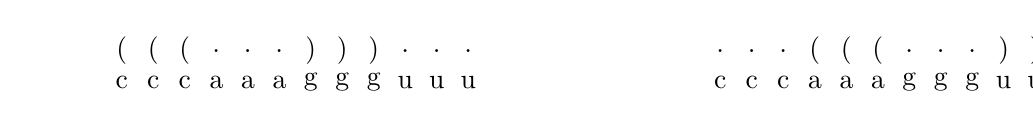
\begin{tikzpicture}[node distance=0.4cm,semithick, main/.style = {draw}]
\tab \node (20) {(}; 
\node (21) [right of=20] {(}; 
\node (22) [right of=21] {(};
\node (23) [right of=22] {.};
\node (24) [right of=23] {.};
\node (25) [right of=24] {.};
\node (26) [right of=25] {)};
\node (27) [right of=26] {)};
\node (28) [right of=27] {)};
\node (29) [right of=28] {.};
\node (30) [right of=29] {.};
\node (31) [right of=30] {.};

\node (1) [below of=20] {c}; 
\node (2) [right of=1] {c};
\node (3) [right of=2] {c};
\node (4) [right of=3] {a};
\node (5) [right of=4] {a};
\node (6) [right of=5] {a};
\node (7) [right of=6] {g};
\node (8) [right of=7] {g};
\node (9) [right of=8] {g};
\node (10) [right of=9] {u};
\node (11) [right of=10] {u};
\node (12) [right of=11] {u};

\node (a) [right of=31] {}; 
\node (b) [right of=a] {}; 
\node (c) [right of=b] {}; 
\node (d) [right of=c] {}; 
\node (e) [right of=d] {}; 
\node (f) [right of=e] {}; 
\node (g) [right of=f] {}; 

\node (40) [right of=g] {.}; 
\node (41) [right of=40] {.}; 
\node (42) [right of=41] {.};
\node (43) [right of=42] {(};
\node (44) [right of=43] {(};
\node (45) [right of=44] {(};
\node (46) [right of=45] {.};
\node (47) [right of=46] {.};
\node (48) [right of=47] {.};
\node (49) [right of=48] {)};
\node (50) [right of=49] {)};
\node (51) [right of=50] {)};

\node (61) [below of=40] {c}; 
\node (62) [right of=61] {c};
\node (63) [right of=62] {c};
\node (64) [right of=63] {a};
\node (65) [right of=64] {a};
\node (66) [right of=65] {a};
\node (67) [right of=66] {g};
\node (68) [right of=67] {g};
\node (69) [right of=68] {g};
\node (70) [right of=69] {u};
\node (71) [right of=70] {u};
\node (72) [right of=71] {u};

\end{tikzpicture} ${\\}$

\textbf{5.}  Donnez un autre arbre de d\'erivation pour la m${\hat{e}}$me s\'eequence et dessinez la structure
secondaire correspondante. \\


\begin{tikzpicture}[node distance=1cm,semithick, main/.style = {draw}]
\tab \tab \tab \node (1) {S}; 
\node (21) [below left of=1] {S}; 
\node (22) [below right of=1] {S};
\node (31) [below of=21] {S}; 
\node (32) [left of=31] {S}; 
\node (33) [below of=22] {S}; 
\node (34) [right of=33] {S}; 
\node (41) [below left of=32] {T}; 
\node (42) [below of=31] {T};
\node (43) [below of=33] {T}; 
\node (44) [below right of=34] {T}; 

\node (51) [below of=41] {T}; 
\node (52) [left of=51] {\textbf{c}}; 
\node (61) [below of=51] {T}; 
\node (62) [left of=61] {\textbf{c}}; 
\node (71) [below of=61] {T}; 
\node (72) [left of=71] {\textbf{c}}; 
\node (81) [below of=71] {${\epsilon}$};

\node (53) [below of=42] {T}; 
\node (54) [left of=53] {\textbf{a}}; 
\node (63) [below of=53] {T}; 
\node (64) [left of=63] {\textbf{a}}; 
\node (73) [below of=63] {T}; 
\node (74) [left of=73] {\textbf{a}}; 
\node (82) [below of=73] {${\epsilon}$};

\node (55) [below left of=43] {\textbf{g}}; 
\node (56) [below right of=43] {T}; 
\node (65) [below of=56] {T}; 
\node (66) [left of=65] {\textbf{g}}; 
\node (75) [below of=65] {T}; 
\node (76) [left of=75] {\textbf{g}}; 
\node (83) [below of=75] {${\epsilon}$};

\node (57) [below of=44] {\textbf{u}}; 
\node (58) [right of=57] {T}; 
\node (67) [below of=57] {\textbf{u}}; 
\node (68) [right of=67] {T}; 
\node (77) [below of=67] {\textbf{u}}; 
\node (78) [right of=77] {T}; 
\node (84) [below of=78] {${\epsilon}$};

\path [->]  (1) edge node {} (21)
(1) edge node {} (22)
(21) edge node {} (31)
(21) edge node {} (32)
(22) edge node {} (33)
(22) edge node {} (34)

(31) edge node {} (42)
(32) edge node {} (41)
(33) edge node {} (43)
(34) edge node {} (44)

(41) edge node {} (51)
(41) edge node {} (52)
(51) edge node {} (61)
(51) edge node {} (62)
(61) edge node {} (71)
(61) edge node {} (72)
(71) edge node {} (81)

(42) edge node {} (53)
(42) edge node {} (54)
(53) edge node {} (63)
(53) edge node {} (64)
(63) edge node {} (73)
(63) edge node {} (74)
(73) edge node {} (82)

(43) edge node {} (55)
(43) edge node {} (56)
(56) edge node {} (65)
(56) edge node {} (66)
(65) edge node {} (75)
(65) edge node {} (76)
(75) edge node {} (83)

(44) edge node {} (57)
(44) edge node {} (58)
(58) edge node {} (67)
(58) edge node {} (68)
(68) edge node {} (77)
(68) edge node {} (78)
(78) edge node {} (84)
\end{tikzpicture} ${\\}$

Structure secondaire correspondante :

\begin{tikzpicture}[node distance=0.4cm,semithick, main/.style = {draw}]
\tab \tab \tab 
\node (20) {.}; 
\node (21) [right of=20] {.}; 
\node (22) [right of=21] {.};
\node (23) [right of=22] {.};
\node (24) [right of=23] {.};
\node (25) [right of=24] {.};
\node (26) [right of=25] {.};
\node (27) [right of=26] {.};
\node (28) [right of=27] {.};
\node (29) [right of=28] {.};
\node (30) [right of=29] {.};
\node (31) [right of=30] {.};

\node (1) [below of=20] {c}; 
\node (2) [right of=1] {c};
\node (3) [right of=2] {c};
\node (4) [right of=3] {a};
\node (5) [right of=4] {a};
\node (6) [right of=5] {a};
\node (7) [right of=6] {g};
\node (8) [right of=7] {g};
\node (9) [right of=8] {g};
\node (10) [right of=9] {u};
\node (11) [right of=10] {u};
\node (12) [right of=11] {u};
\path [-]  (1) edge node {} (2)
(2) edge node {} (3)
(3) edge node {} (4)
(4) edge node {} (5)
(5) edge node {} (6)
(6) edge node {} (7)
(7) edge node {} (8)
(8) edge node {} (9)
(9) edge node {} (10)
(10) edge node {} (11)
(11) edge node {} (12)
\end{tikzpicture} ${\\}$


\textbf{6.}  On consid\`ere pour cette question que les appariements possibles dans une structure
secondaire d\textquoteright ARN sont les appariements canoniques a-u, u-a, c-g et g-c, ainsi que
les appariements dits “wobble” g-u et u-g. \\

\textit{(a)}  Soit L${_0}$ le plus grand langage sur l\textquoteright alphabet \{a, c, g, u\} qui poss\`ede la propri\'et\'e suivante : quel que soit \textit{w}  ${\epsilon}$ L${_0}$, il n\textquoteright y a aucun appariement possible dans \textit{w}. Donnez une expression rationnelle et un automate fini pour L${_0}$. \\

Expression rationnelle de L${_0}$ : \\

(a | c)${^*}$ | (a | g)${^*}$ | (u | c)${^*}$ | (u | g)${^*}$ \\

Automate fini de L${_0}$ : \\

\begin{tikzpicture}[node distance=1.7cm,semithick, main/.style = {draw, circle}]
\tab \tab \tab 
\node[main] (0) {0}; 
\node (10) [right of=0] {}; 
\node[main] (1) [above right of=10] {1}; 
\node[main] (2) [below right of=10] {2};
\node[main] (3) [above of=1] {3}; 
\node[main] (4) [below of=2] {4};
\node (11) [right of=1] {}; 
\node (12) [right of=2] {}; 
\node (13) [right of=3] {}; 
\node (14) [right of=4] {}; 
\node (15) [left of=0] {}; 

\path [->]  (0) edge node {${\epsilon}$} (1)
(0) edge node {${\epsilon}$} (2)
(0) edge node {${\epsilon}$} (3)
(0) edge node {${\epsilon}$} (4)
(1) edge [loop above] node {a,c} (1)
(2) edge [loop above] node {a,g} (2)
(3) edge [loop above] node {u,c} (3)
(4) edge [loop above] node {u,g} (4)
(15) edge node {} (0)
(1) edge node {} (11)
(2) edge node {} (12)
(3) edge node {} (13)
(4) edge node {} (14)

\end{tikzpicture} ${\\}$

\textit{(b)}  Soit L${_1}$ le plus grand langage sur l\textquoteright alphabet \{a, c, g, u\} qui poss\`ede la propri\'et\'e suivante : quel que soit \textit{w} ${\epsilon}$ L${_1}$, il y a exactement un appariement possible dans
\textit{w} . Donnez une expression rationnelle et un automate fini pour L${_1}$ . \\

Expression rationnelle de L${_0}$ : \\

(c | g | a)${^*}$ a (c | g | a)${^*}$ u (c | g | a)${^*}$  | (c | g | u)${^*}$ a (c | g | u)${^*}$ u (c | g | u)${^*}$  | \\
\tab (c | g | a)${^*}$ u (c | g | a)${^*}$ a (c | g | a)${^*}$  | (c | g | u)${^*}$ u (c | g | u)${^*}$ a (c | g | u)${^*}$  | \\
\tab (c | u | a)${^*}$ g (c | u | a)${^*}$ c (c | u | a)${^*}$  | (a | g | u)${^*}$ g (a | g | u)${^*}$ c (a | g | u)${^*}$  | \\
\tab (c | u | a)${^*}$ c (c | u | a)${^*}$ g (c | u | a)${^*}$  | (a | g | u)${^*}$ c (a | g | u)${^*}$ g (a | g | u)${^*}$ \\



Automate fini de L${_0}$ : \\

\end{document}

